\documentclass{beamer}
\usetheme{simple}

\usepackage{amsmath}
\usepackage[export]{adjustbox}
\usepackage{graphicx}
\usepackage{lmodern}
\usepackage{transparent}
\usepackage[scale=2]{ccicons}

\setbeamercovered{invisible}

\title{Bayes Workshop 1}
\subtitle{Bayesian Probability and the Likelihood Function}
\date{\today}
\author{Corson N. Areshenkoff}
\institute{University of Victoria}

\begin{document}

\maketitle

\begin{frame}{The Problem}
Find a coin on the sidewalk. How do we know if the coin is fair? \par
In other words, we want to know the probability $p$ that a coin returns heads.
\end{frame}

\begin{frame}{The Problem}
How do we get $p$?
        \begin{itemize}
                \item First, specify a probability model. 
                \begin{itemize}
                        \item If a coin flip is random, what is its distribution?
                        \item If we flip the coin repeatedly, how many heads should we see?
                \end{itemize}     
                \item Then, collect data
                \begin{itemize}
                        \item Flip the coin many times and observe the proportion of heads.
                        \item The number of heads obtained in $N$ independent flips of a coin is a \emph{binomial} random variable.
                \end{itemize}                                           
        \end{itemize}
\end{frame}

\begin{frame}{Probability Mass Function}
\begin{itemize}
        \item The \emph{probability mass function} (pmf) of a (discrete) random variable gives the probability of observing an outcome $x$.
        \item For $N$ coin flips (with probability $p$ of heads), the pmf gives the probability of observing $k$ heads.
\end{itemize}        
\end{frame}

\begin{frame}{Probability Mass Function}
How do we get the pmf? \par Suppose we flip a fair coin 4 times ($N=4, p = 0.5$). What is the probability that we get ONE head?
        \begin{itemize}
                \item The head happens with probability $\frac{1}{2}$
                \item Each tails happens with probability $\frac{1}{2}$, giving
                         $\left ( \frac{1}{2} \right )^3$
                \item \dots but there are $4$ places the head can appear.
        \end{itemize}
So the probability is 
        \[
                P(1;N=4,p=0.5) = 
                        4 \left ( \frac{1}{2} \right ) \left ( \frac{1}{2} \right )^3
        \]
\end{frame}

\begin{frame}{Probability Mass Function}
In general, the binomial pmf is given by
                \[
                P(k;N,p) = \underbrace{{n \choose k}}_{\text{\# of ways}}
                                \overbrace{p^k}^{\text{k heads}}
                                \underbrace{(1-p)^{n-k}}_{\text{n-k tails}}
                \]
\end{frame}

% Likelihood
\begin{frame}{Likelihood}
        \begin{itemize}
                \item When we flip a fair coin $N$ times, we talk about the \emph{probability} of observing $k$ heads ($N$ and $p$ are fixed parameters; the \emph{outcome} is unknown).
                        \begin{itemize}
                                \item Probability mass function $P(k;N,p)$
                        \end{itemize}
                \item After performing the experiment and \emph{observing} $k$ heads, we can treat $p$ as unknown and ask: what is the probability that a specific value of $p$ would give us $k$ heads? (what is the \emph{likelihood} that $p$ takes a specific value?)
                        \begin{itemize}
                                \item Likelihood function $\mathcal{L}(p;N,k)$
                        \end{itemize}
        \end{itemize}
\end{frame}

\begin{frame}{Likelihood}
A practical example:
        \begin{itemize}
                \item Flip a coin $4$ times and observe $3$ heads. Which value of $p$ is
                         most likely?
                \item For $p = 0$, the probability of observing $3$ heads is zero, so
                          so the likelihood that $p=0$ is zero.
                \item For $p = 1/2$, the probability of observing $3$ heads is $0.25$, so
                          so the likelihood that $p=1/2$ is $1/4$.
                \item For $p = 3/4$, the probability of observing $3$ heads is $0.43$, so
                          so the likelihood that $p=3/4$ is $0.43$.
                          \begin{itemize}
                                  \item This is the value of $p$ with the \emph{highest} 
                                            likelihood. In other words, $p = 3/4$ maximizes the 
                                            probability of obtaining our data.
                          \end{itemize}
        \end{itemize}
\end{frame}

\begin{frame}{The Likelihood Function}
        \begin{itemize}
                \item Every statistical model (regression, distribution fitting, etc) produces
                          a \emph{likelihood function}, which gives the probability of 
                          obtaining a set of data for different values of the model parameters.
                \item If $D$ are the data, and $\Theta$ are the parameters of the model 
                         (say, regression coefficients), then
                                 \[ \mathcal{L}(\Theta|D) = P(D|\Theta) \]
                \item Common practice is to choose the parameters values which 
                          maximize the likelihood function (i.e. which maximize the 
                          probability of obtaining the observed data).
                          \begin{itemize}
                                  \item This is \emph{maximum likelihood estimation}, and the
                                            resulting parameter estimates are called the 
                                            \emph{maximum likelihood estimates} (MLE's)
                          \end{itemize}
        \end{itemize}
\end{frame}

\begin{frame}{The Likelihood Function}
Some examples:
        \begin{itemize}
                \item The MLE for $p$ in our coin flip example
                          is the observed proportion of heads $\hat{p} = k/N$.
                \item The MLE's for the mean and variance of a normal distribution are
                        \begin{align*}
                                \hat{\mu} &= \bar{X} = \frac{\sum_{i=1}^N x_i}{N} \\
                                \hat{\sigma}^2 &= \frac{\sum_{i=1}^N (\bar{X} - x_i)^2}{N}
                        \end{align*}
                \item The MLE's for a linear regression model are the usual least squares
                          estimates.
        \end{itemize}
\end{frame}

\begin{frame}{The Likelihood Function}
        \begin{itemize}
                \item The likelihood function is, arguably, the most important concept in
                          statistical inference.
                \item \textbf{All of the information contained in the data about a model is 
                               contained in the likelihood function}.
                \item In practice, the natural logarithm of the likelihood function
                         (the log-likelihood) is usually easier to work with.
        \end{itemize}
\end{frame}


% Bayes
\begin{frame}{Bayesian Probability}
What does probability mean? 
    \begin{itemize}
        \item "A coin flip has a \%50 chance of landing on heads"
            \begin{description}
                \item[Frequentist] If we flip the coin a large number of times, approximately
                        half of the coin flips will be heads.
                \item[Bayesian] If we're asked to call a coin flip, we have no reason to 
                        prefer heads or tails.
            \end{description}
\textbf{Frequentists} define probability in terms of long-run averages.\par
\textbf{Bayesians} define probability in terms of degrees of belief. 
    \end{itemize}
\end{frame}

\begin{frame}{Bayesian Estimation}
Suppose that we pick up a newly minted coin and flip it $N=4$ times, obtaining $k=3$ heads.
The MLE for the probability $p$ is $k/N = 0.75$.\par
Which is more plausible?
    \begin{itemize}
        \item The finely tuned machines used to mint the coin made a mistake, and somehow minted a  highly unbalanced coin.
        \item The coin is fair, but just happened to return 3 heads.
    \end{itemize}
\end{frame}

\begin{frame}{Bayesian Estimation}
    \begin{enumerate}
        \item Decide on a model (a set of distribution that characterize the data)
        \item Specify prior distributions for the model parameters
        \item Use data to update the prior distributions (w/ likelihood)
        \item Obtain posterior
    \end{enumerate}
\end{frame}

\begin{frame}{Bayesian Estimation}
Or, more rigorously...
    \begin{enumerate}
        \item Define a statistical model with parameters $\Theta$.
        \item Model gives a likelihood function $\mathcal{L}(\Theta|D) = p(D|\Theta)$, which     
              summarizes the evidence contained in the data.
        \item Specify a prior distribution $p(\Theta)$, which summarizes our prior belief
              about the parameters.
        \item Combine the likelihood and the prior to get a posterior distribution
              $p(\Theta|D)$.
              \[ p(\Theta|D) \propto p(D|\Theta)p(\Theta) \]
              which summarizes our new belief about the parameter, after taking into account
              the data.
    \end{enumerate}
\end{frame}

\begin{frame}
    \begin{figure}
    \centering
        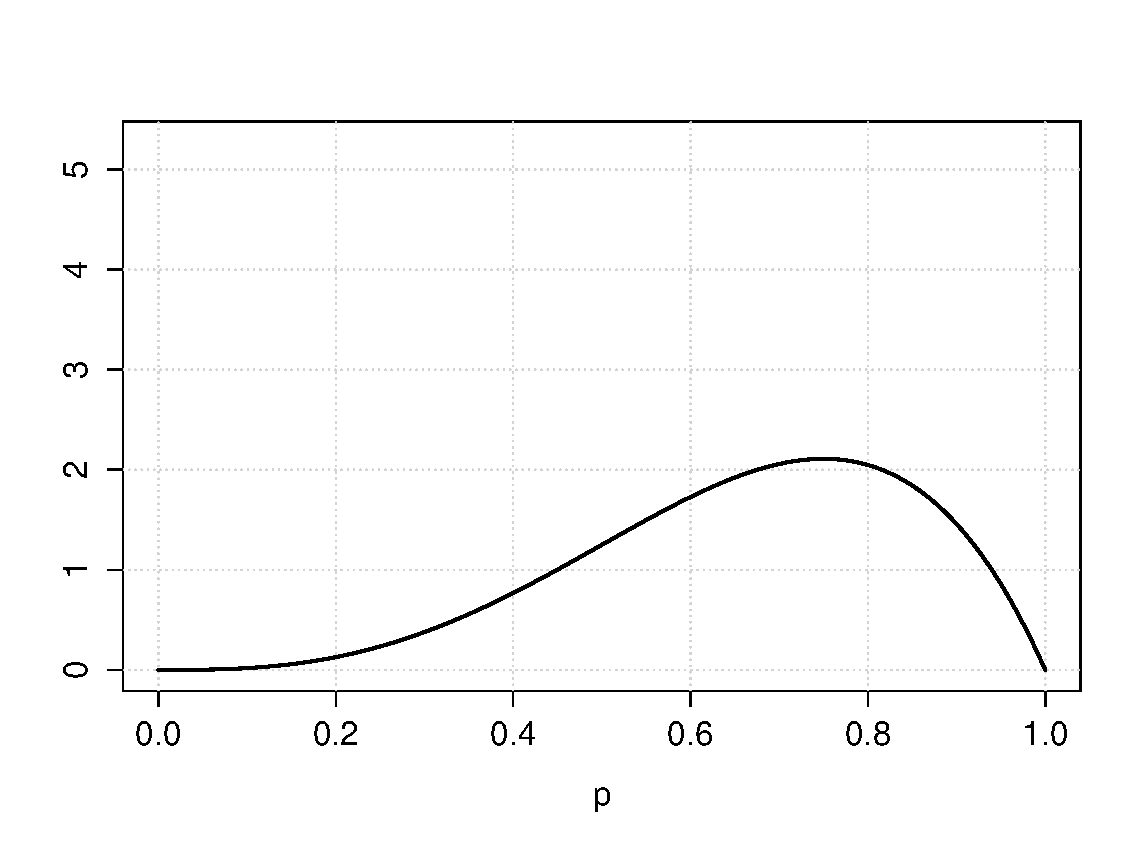
\includegraphics[width=.8\textwidth]{../images/binom_likelihood.pdf}
        \caption{Binomial likelihood function for $N=4$ and $k=3$.}
    \end{figure}
\end{frame}

\begin{frame}
    \begin{figure}
    \centering
        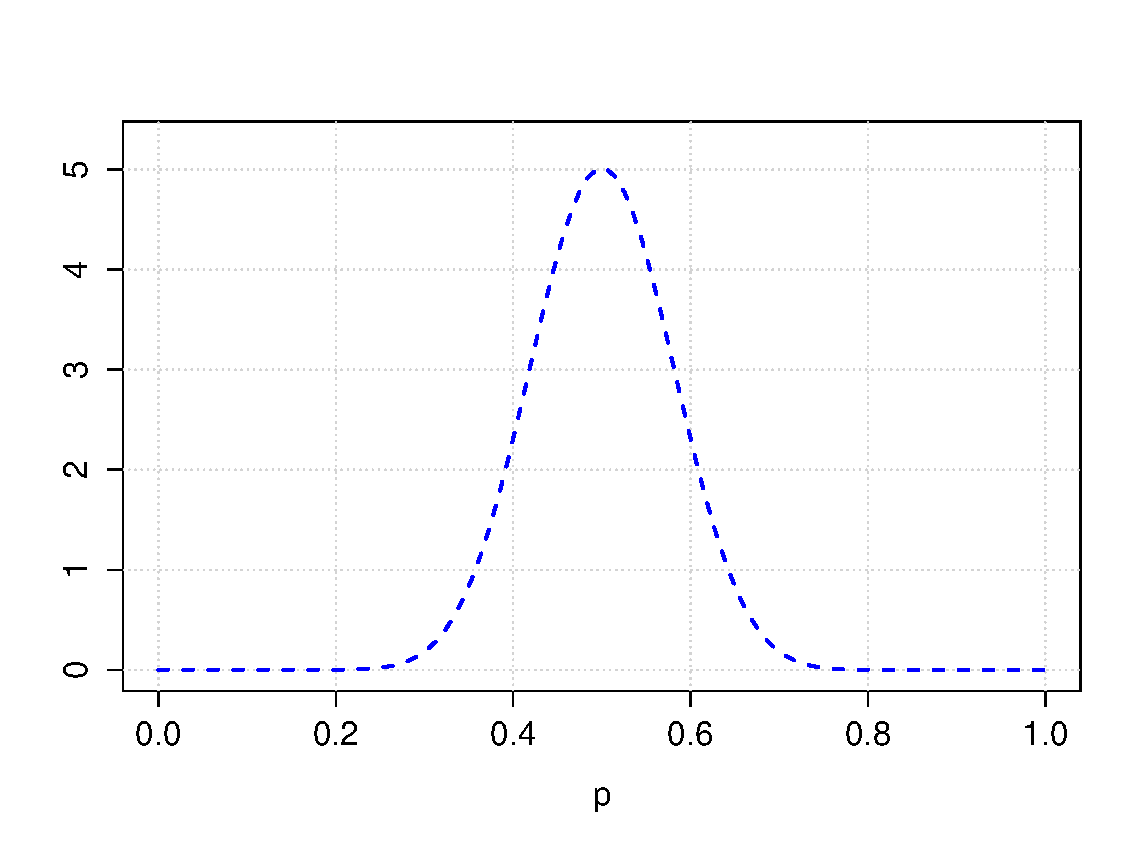
\includegraphics[width=.8\textwidth]{../images/binom_prior.pdf}
        \caption{Beta(20,20) prior distribution for binomial parameter $p$.}
    \end{figure}
\end{frame}

\begin{frame}
    \begin{figure}
    \centering
        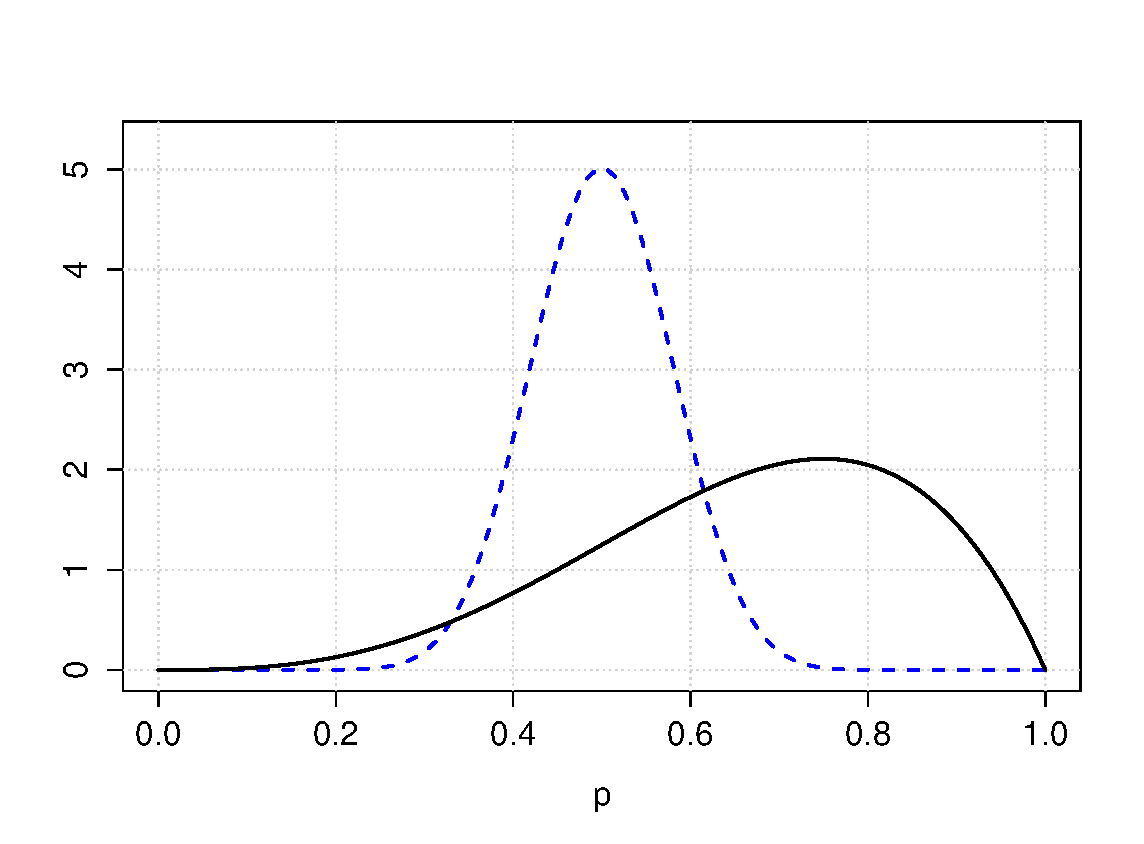
\includegraphics[width=.8\textwidth]{../images/binom_prior_likelihood.pdf}
        \caption{Likelihood and prior together.}
    \end{figure}
\end{frame}

\begin{frame}
    \begin{figure}
    \centering
        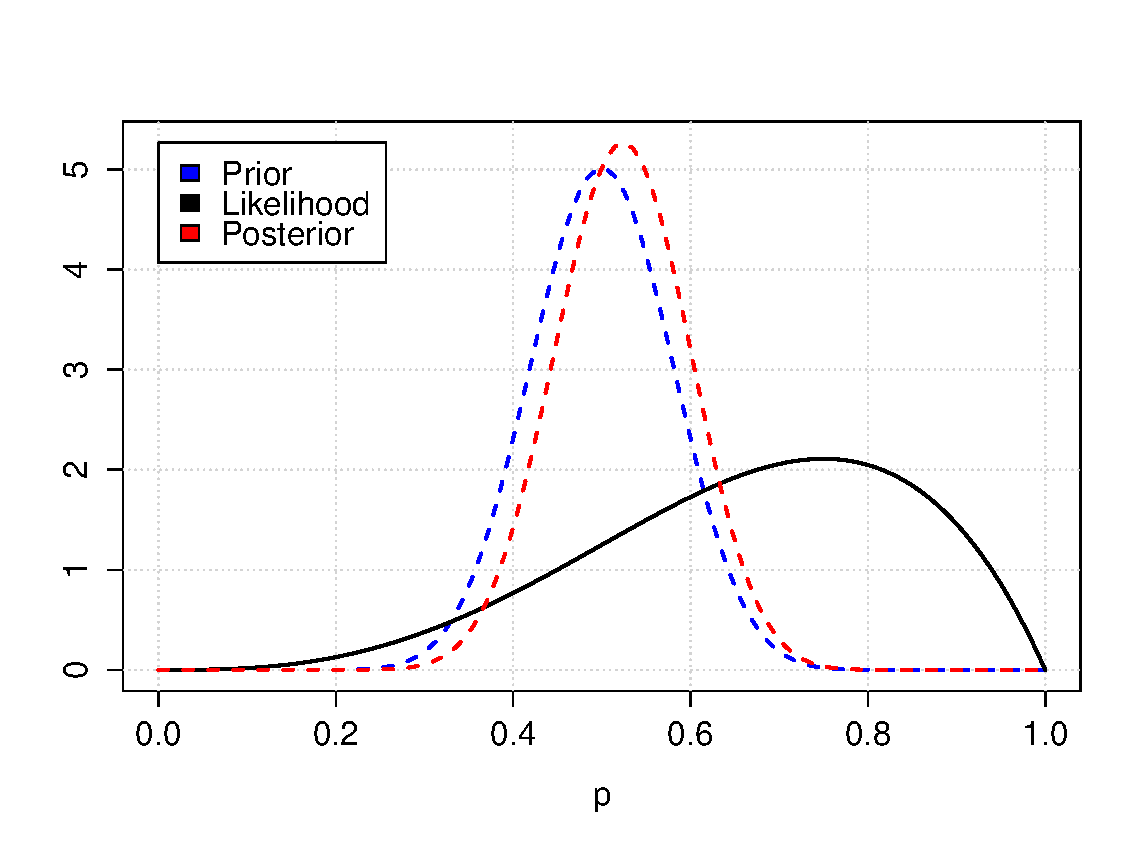
\includegraphics[width=.8\textwidth]{../images/binom_posterior.pdf}
        \caption{Relationship between prior, likelihood, and posterior distribution.}
    \end{figure}
\end{frame}



% Fitting models in STAN
\begin{frame}
In general, computing posterior distributions is difficult or impossible, so we have to approximate them using e.g. MCMC. \par

There are several software packages to do this (e.g. BUGS, JAGS, Stan). \par 

We use Stan, for reasons that we'll get into next time.
\end{frame}

\begin{frame}[fragile]
The \textbf{data} block specifies the data that will be passed to Stan:
\begin{verbatim}
    data {
        int<lower=0> N; // Number of coin flips
        int k;          // Number of heads
    }
\end{verbatim}
\end{frame}

\begin{frame}[fragile]
The \textbf{parameters} block specifies the parameters of our model:
\begin{verbatim}
    parameters {
        real<lower=0, upper = 1> p;
    }
\end{verbatim}
\end{frame}

\begin{frame}[fragile]
The \textbf{model} block specifies the likelihood/priors:
\begin{verbatim}
    model {
        h ~ binomial(N, p);  // Likelihood
        p ~ beta(1,1);       // Prior
    }
\end{verbatim}
\end{frame}

\begin{frame}[fragile]
The complete .stan file is then:
\begin{verbatim}
    data {
        int<lower=0> N; // Number of coin flips
        int k;          // Number of heads
    }
    
    parameters {
        real<lower=0, upper = 1> p;
    }
    
    model {
        h ~ binomial(N, p);  // Likelihood
        p ~ beta(1,1);       // Prior
    }
\end{verbatim}
\end{frame}

\end{document}